%*****************************************
\chapter{Experiments}\label{ch:experiments}
%*****************************************

\section{Blocks World as a Simple Real-Time Symbolic Control Problem Domain}

\begin{figure}[bth]
  \center
  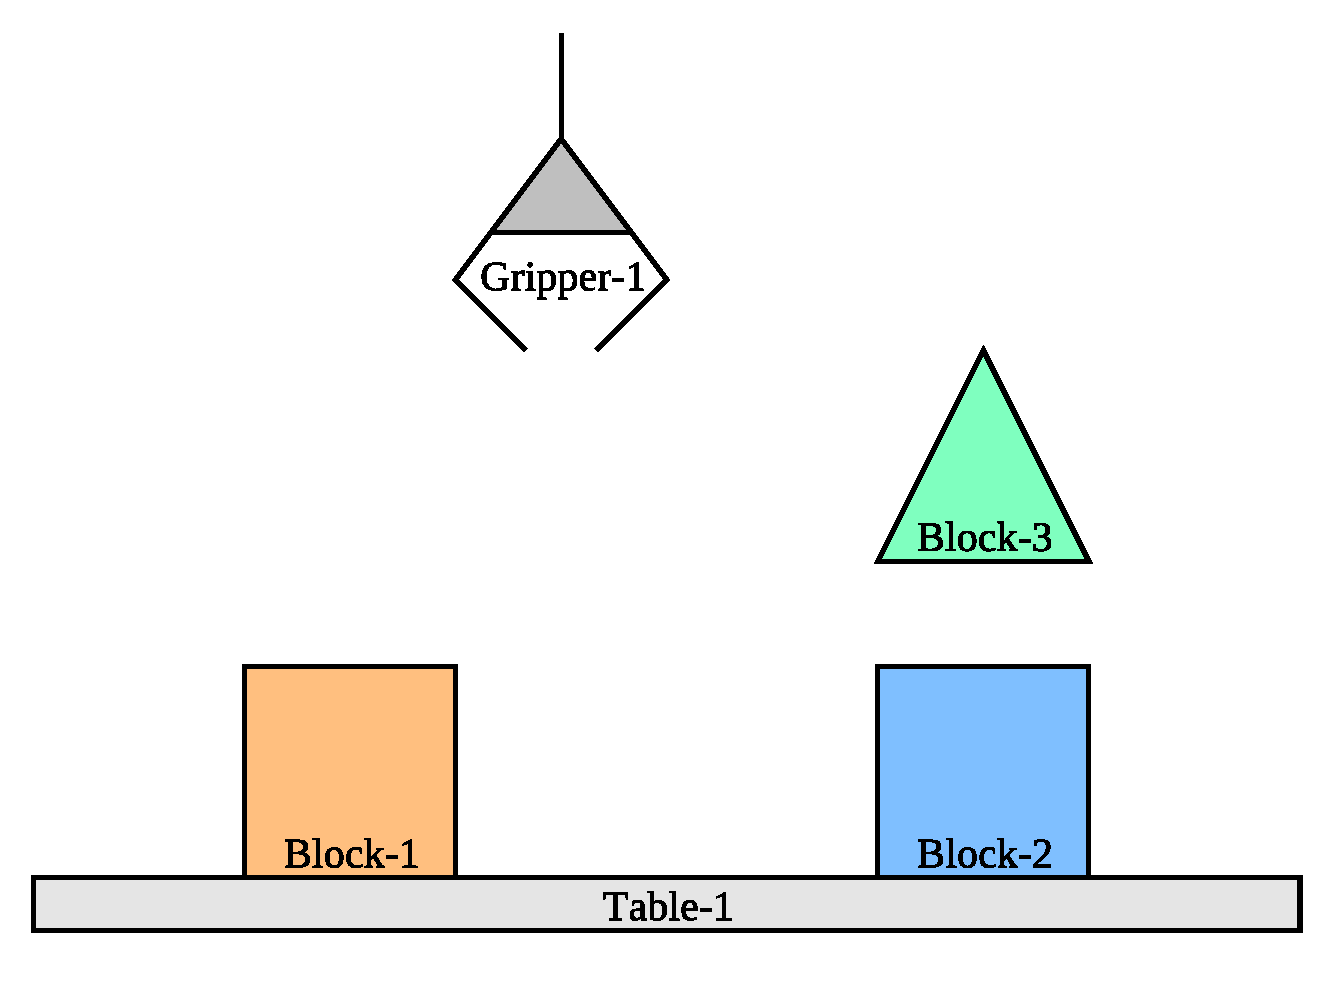
\includegraphics[width=11cm]{gfx/blocks_world_screenshot-1}
  \caption[Blocks world is a simple real-time symbolic control problem.]{Blocks world is a simple real-time symbolic control problem that I use to demonstrate my reflective control learning theory.}
  \label{fig:blocks_world_screenshot-1}
\end{figure}

I use blocks world, a canonical toy AI problem, in order to demonstrate my example of reflectively learning to plan.
See Figure~\ref{fig:blocks_world_screenshot-1} for a screenshot of my blocks world problem physical simulation.

\begin{table}
  \myfloatalign
  \begin{tabularx}{\textwidth}{XllX}
    & [Gripper-1 is me] & [Gripper-1 movement\_command []] & \\
    & [Gripper-1 is-a gripper] & [Gripper-1 color black] & \\
    & [Gripper-1 is-holding []] & [Block-1 is-a block] & \\
    & [Block-1 color brown] & [Block-1 shape cube] & \\
    & [Block-1 on Table-1] & [Block-1 left-of Gripper-1] & \\
    & [Block-2 is-a block] & [Block-2 color blue] & \\
    & [Block-2 shape cube] & [Block-2 on Table-1] & \\
    & [Block-2 right-of Gripper-1] & [Block-3 is-a block] & \\
    & [Block-3 color green] & [Block-3 shape pyramid] & \\
    & [Block-3 right-of Gripper-1] & [Table-1 is-a block] & \\
    & [Table-1 color white] & [Table-1 shape cube] & \\
    & [Table-1 left-of Gripper-1] & &
  \end{tabularx}
  \caption[Blocks world agent perceptual input.]{Blocks world agent perceptual input.}
  \label{tab:blocks_world_agent_perceptions}
\end{table}

See Table~\ref{tab:blocks_world_agent_perceptions} for an example set of perceptual input that corresponds with the physical situation shown in Figure~\ref{fig:blocks_world_screenshot-1}.

\section{Working in a World of Building Blocks}

In his PhD thesis, Terry Winograd worked in the world of building
blocks \citep{winograd:1970}.  This program maintained traces of its
goals and subgoals, which enabled it to answer questions about why it
performed certain actions.  This system worked because it stored
goals.

Knowing the goal state of the computation is important, and I do not
ignore this aspect in tracing the deliberative layer.  My system is
able to answer these sorts of questions, as this simply requires
climbing the stack of mental resource activations, but when debugging
the deliberative process, it is helpful to not only know the ending
point of computation but also the means toward that end.

\section{Terry Winograd's SHRDLU and Goal Tracing}

I am building upon what was learned from Winograd's thesis
\citep{winograd:1970} in terms of using traces of the deliberative
process as well as using a semantic model of the world in order to
understand communications between agents.  I have chosen to use a
simpler and more direct language interface between agents that refers
more directly to the semantic information and mental processes
involved.  I have experimented with implementing the original SHRDLU
english language parser, although I believe the parsing process can be
better controlled as a goal-oriented set of concurrent processes than
as the stack-based depth first search that I started writing in my
initial experiments.

\section{Why Not Work Solely Within the Blocks World Domain?}

The building blocks approach is a good precedent.  However, there are
many problems with only demonstrating a solution on a toy problem.
First, an approach demonstrated to solve a small problem, often do not
scale to larger problem domains of similar complexity.  So, I feel
that it is important to show the same reflective approach to learning
can also be applied to a domain with a much larger state space than
the toy blocks world problem.  I then, have shown the theoretical
gains of my approach by using the canonical model as a tool for
explanation, and now I show that my model does scale to larger
problem domains of only slightly more complexity.  See
\cite{smith:2010} for a discussion of the benefits of approaching the
social commonsense reasoning problem with a physical simulation of a
kitchen.

I have conscripted my domain of object types in the kitchen, such
that it is currently comparable to the number of object types that
Winograd used in his thesis.  My object types do have different ways
that they may be used, which is a small addition of complexity.
Although I do not introduce many of the complexities of ontological
reasoning, a common approach to commonsense reasoning, e.g. Cyc
\citep{lenat:1990}, my system demonstrates an important new approach
to commonsense reasoning that grounds learning by being told in the
domain of goal-oriented reasoning, which allows organizing and
debugging knowledge in terms of what goals it is useful for
accomplishing.

\section{A Physical Simulation of a Kitchen as a Social Commonsense Reasoning Domain}

\begin{figure}[bth]
  \center
  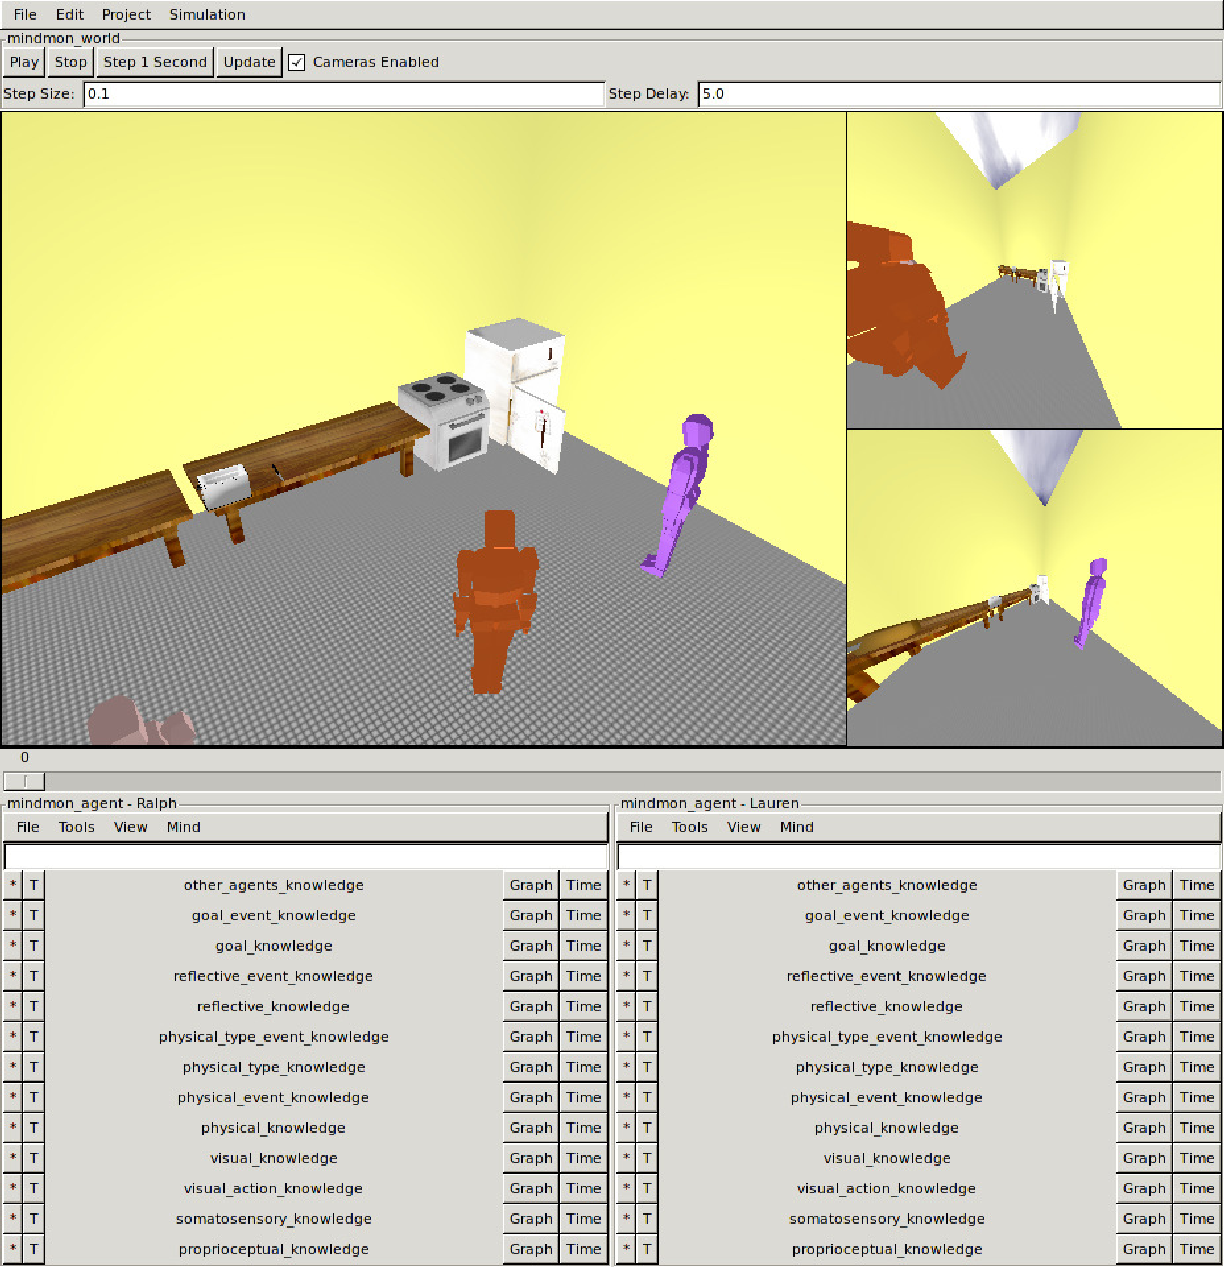
\includegraphics[width=11cm]{gfx/mindmon-isis_world-screenshot-1}
  \caption[Isis World is a larger physical simulation than the Blocks
    World toy problem.]{Isis World is a larger real-time symbolic
    physical simulation, which I use to demonstrate that my reflective
    goal-oriented learning approach scales to the physical and
    reflective problem spaces of slightly more complicated learning
    problems.}
  \label{fig:mindmon-isis_world-screenshot-1}
\end{figure}

I have experimented with applying my cognitive architecture to a
larger social commonsense reasoning domain with parents that teach
children as they attempt to accomplish cooking tasks in a kitchen.
See \cite{morgan:2011} for details about my six-layered reflective
theory of social and moral reasoning, which assumes the existence of a
procedurally reflective infrastructure with a reflective problem
solver written within it.

\section{Why is Cooking in a Kitchen a Good Problem to Model?}

\cite{smith:2010} discuss reasons for why focusing on solving cooking
tasks in a kitchen will lead to a better understanding of the
reflective control of multiple agents in a common complicated social
environment.  Further, \cite{morgan:2010} describes how focusing on
this domain from a reflective architectural point of view can lead to
future models of self-reflective and self-conscious learning between
parents and children.

From an educational perspective, \cite{dewey:1907} has
theorized that kitchens are a good example of a rich learning
environment for children.  Some form of kitchen, or a social place
where food is cooked for a family, is ubiquitous across cultures.
Kitchens have a clear production goal, namely food.  Many mental
realms must be used in accomplishing even simple cooking goals,
including: math, physics, chemistry, thermodynamics, language,
society, family, imprimer learning, concurrent planning, etc.  See
Figure~\ref{fig:mindmon-isis_world-screenshot-1} for a screenshot of
my graphical user interface to the cognitive architecture, while it
interacts with the Isis World physical simulation.

